% Options for packages loaded elsewhere
\PassOptionsToPackage{unicode}{hyperref}
\PassOptionsToPackage{hyphens}{url}
%
\documentclass[
]{article}
\usepackage{lmodern}
\usepackage{amssymb,amsmath}
\usepackage{ifxetex,ifluatex}
\ifnum 0\ifxetex 1\fi\ifluatex 1\fi=0 % if pdftex
  \usepackage[T1]{fontenc}
  \usepackage[utf8]{inputenc}
  \usepackage{textcomp} % provide euro and other symbols
\else % if luatex or xetex
  \usepackage{unicode-math}
  \defaultfontfeatures{Scale=MatchLowercase}
  \defaultfontfeatures[\rmfamily]{Ligatures=TeX,Scale=1}
\fi
% Use upquote if available, for straight quotes in verbatim environments
\IfFileExists{upquote.sty}{\usepackage{upquote}}{}
\IfFileExists{microtype.sty}{% use microtype if available
  \usepackage[]{microtype}
  \UseMicrotypeSet[protrusion]{basicmath} % disable protrusion for tt fonts
}{}
\makeatletter
\@ifundefined{KOMAClassName}{% if non-KOMA class
  \IfFileExists{parskip.sty}{%
    \usepackage{parskip}
  }{% else
    \setlength{\parindent}{0pt}
    \setlength{\parskip}{6pt plus 2pt minus 1pt}}
}{% if KOMA class
  \KOMAoptions{parskip=half}}
\makeatother
\usepackage{xcolor}
\IfFileExists{xurl.sty}{\usepackage{xurl}}{} % add URL line breaks if available
\IfFileExists{bookmark.sty}{\usepackage{bookmark}}{\usepackage{hyperref}}
\hypersetup{
  pdftitle={Bayesian Mixture Cure Modelling in Metastatic Melanoma (CheckMate 067)},
  pdfauthor={N Green, UCL},
  hidelinks,
  pdfcreator={LaTeX via pandoc}}
\urlstyle{same} % disable monospaced font for URLs
\usepackage[margin=1in]{geometry}
\usepackage{graphicx}
\makeatletter
\def\maxwidth{\ifdim\Gin@nat@width>\linewidth\linewidth\else\Gin@nat@width\fi}
\def\maxheight{\ifdim\Gin@nat@height>\textheight\textheight\else\Gin@nat@height\fi}
\makeatother
% Scale images if necessary, so that they will not overflow the page
% margins by default, and it is still possible to overwrite the defaults
% using explicit options in \includegraphics[width, height, ...]{}
\setkeys{Gin}{width=\maxwidth,height=\maxheight,keepaspectratio}
% Set default figure placement to htbp
\makeatletter
\def\fps@figure{htbp}
\makeatother
\setlength{\emergencystretch}{3em} % prevent overfull lines
\providecommand{\tightlist}{%
  \setlength{\itemsep}{0pt}\setlength{\parskip}{0pt}}
\setcounter{secnumdepth}{-\maxdimen} % remove section numbering

\title{Bayesian Mixture Cure Modelling in Metastatic Melanoma (CheckMate
067)}
\author{N Green, UCL}
\date{14/10/2020}

\begin{document}
\maketitle

{[}taken from Anthonio{]}

\hypertarget{methodology}{%
\subsubsection{Methodology}\label{methodology}}

Immuno-oncologic (IO) studies for melanoma therapies, such as
\emph{ipilimumab}, \emph{nivolumab}, and the \emph{nivolumab} +
\emph{ipilimumab} combination, have indicated that survival curves
``plateau'' (a considerable proportion of patients are ``long-term
survivors''). Cure models are a special type of survival analysis where
this ``cure fraction'' (the underlying proportion of responders to
treatment/long-term survivors) is accounted for. Cure models estimate
the cure fraction, in addition to a parametric survival function for
patients that are not cured. The mortality risk in the cured patients is
informed by a background mortality rate. The population that is not
cured is subject both to background mortality and to additional
mortality from their cancer, estimated using a parametric survival
model.

A mixture cure model (MCM) is a type of cure model where survival is
modelled as a mixture of two groups of patients: those who are cured and
those who are not (and who therefore remain at risk). The survival for a
population with a cure fraction can be written as follows:

\begin{equation}
S(t, x) = S^*(t, x)[\pi(x) + (1 − \pi(x))S_u(t, x)],
\end{equation}

where \(S(t, x)\) denotes the survival at time \(t\), \(S^*(t, x)\)
denotes the background mortality at time \(t\) conditional on covariates
\(x\), \(\pi(x)\) denotes the probability of being cured conditional on
covariates \(x\), and \(S_u(t, x)\) denotes the mortality due to cancer
at time t conditional on covariates \(x\). We use World Health
Organization (WHO) life tables by country (2018) to inform the
background mortality rate (baseline hazard) inputed to the cure model.
Such baseline hazard is the expected mortality rate for each patient at
the age at which he/she experiences the event. The mortality data are
age- and gender adjusted, thus providing a granular account of the
different patient profiles in the trial. Note that WHO reports
conditional probabilities of death in 5-year intervals until age 85. A
constant annual mortality rate is reported for individuals over 85. In
addition, we make the assumption that the maximum age that a patient can
live up to is 100 years.

To model the disease-specific mortality (the uncured fraction), all
standard parametric distributions are tested:

\begin{itemize}
\tightlist
\item
  exponential
\item
  Weibull
\item
  Gompertz
\item
  log-normal
\item
  log-logistic
\item
  generalised gamma.
\end{itemize}

Parameters for the models, including the cure rate parameter, are
derived via Bayesian inference.

\hypertarget{model-description}{%
\subsubsection{Model description}\label{model-description}}

Let \(T_i\) be the non-negative random variable denoting the survival
time of patient \(i\) with covariate vector \(\boldsymbol{x}_i\).

We can assume that the cure fraction is the same for the whole
population i.e.~\(\pi\) is fixed. Further, we can assume the \(\pi\)
models the relationship between \(\boldsymbol{x}_i\) and the probability
of being cured. E.g. using a logistic-linear model

\[
\pi(\boldsymbol{x}_i | \boldsymbol{\beta}) = 1/[1 + \exp(-\boldsymbol{x}_i^T \boldsymbol{\beta})].
\]

The likelihood of the standard survival is

\[
L = \prod_i S(t_i | \boldsymbol{x}_i) h(t_i | \boldsymbol{x}_i)^{\delta_i}
\]

Log-likelihood \[
\mathcal{l} = \sum_i \log(S(t_i | \boldsymbol{x}_i)) + \delta_i \log(h(t_i | \boldsymbol{x}_i))
\]

Using this with the mixture cure equation gives

\[
\mathcal{l}(\pi | \boldsymbol{\delta}, \boldsymbol{x}) =
 \sum_i \log(S^*(t_i | \boldsymbol{x}_i) h^*(t_i | \boldsymbol{x}_i)^{\delta_i}[\pi(x) +
   (1 − \pi(x)) S_u(t_i | \boldsymbol{x}_i) h_u(t_i | \boldsymbol{x}_i)^{\delta_i}])
\]

Posterior distribution with cure fraction independent on covariates.

\[
p(\pi, \boldsymbol{\beta^u}, \boldsymbol{\beta^*} | \boldsymbol{\delta}, \boldsymbol{x}) \propto L(\pi, \boldsymbol{\beta^u}, \boldsymbol{\beta^*} | \boldsymbol{\delta}, \boldsymbol{x}) f(\pi) g_2(\boldsymbol{\beta^u}) g_3(\boldsymbol{\beta^*})
\]

Cure fraction dependent on covariates.

\[
p(\pi, \boldsymbol{\beta^u},\boldsymbol{\beta^*}, \boldsymbol{\beta^{cf}} | \boldsymbol{\delta}, \boldsymbol{x}) \propto L(\pi, \boldsymbol{\beta^u},\boldsymbol{\beta^*}, \boldsymbol{\beta^{cf}} | \boldsymbol{\delta}, \boldsymbol{x}) g_1(\boldsymbol{\beta^{cf}})  g_2(\boldsymbol{\beta^u}) g_3(\boldsymbol{\beta^*})
\]

\hypertarget{exponential}{%
\subsubsection{Exponential}\label{exponential}}

Define \(f(t)\) density, \(S(t)\) survival and \(h(t)\) hazard
functions.

\[
f(t) = \lambda \exp(-\lambda t), \;\; S(t) = \exp(-\lambda t), \;\; h(t) = \lambda
\]

Which gives the likelihood

\[
\mathcal{l}(\pi | \boldsymbol{\delta}, \boldsymbol{x}) =
 \sum_i \log(\exp(-\lambda^* t) \lambda^{* \delta}[\pi(x) +
   (1 − \pi(x)) \exp(-\lambda_u t) \lambda_u^{\delta_i}])
\]

\hypertarget{prior-specification}{%
\paragraph{Prior specification}\label{prior-specification}}

The marginal prior distributions will probably depend on which group of
data are being modelled.

\begin{itemize}
\tightlist
\item
  \emph{Cure fraction}
\end{itemize}

We can specify directly using a Beta(\(a\), \(b\)) prior, most
uninformative at a uniform Beta(1,1). Incorporating the covariate via a
logistic link we specify priors on the linear coefficient
\(\beta^{cf}_0, \beta^{cf}_1\). Although not strictly recommended, we
could take sensible starting values from the previous frequentist
analysis results. For example, for OS the nivo, ipi and combined mean
cure fractions were 45\%, 23\% and 54\%. If the data are centred then
this corresponds to \(\beta^{cf}_0 = -0.2, -1.2, 0.16\), respectively.
We would still need to specify how much we expect one year increase in
age would change the cure fraction.

\begin{itemize}
\tightlist
\item
  \emph{Background survival}
\end{itemize}

The default survival curves used in this analysis are from country-level
WHO data. We can consider these to provide sufficiently accurate
estimates given the sample size and so incorporating uncertainty is not
necessary. In fact these annual point estimates are used directly in the
frequentist analysis. This is done by age matching each individual with
the life table and then obtaining the mortality rate at the event time.

However, we also want the developed model to be able to be applied to
other datasets which may be smaller or noisy. Sensible prior parameter
values can be taken for the life table hazard curve. After infancy the
log-hazard is approximately linear and so intercept and slope estimates
are simple to obtain.

\begin{itemize}
\tightlist
\item
  \emph{Mortality due to cancer}
\end{itemize}

\hypertarget{initial-results}{%
\subsubsection{Initial results}\label{initial-results}}

We fit the exponential hazard model to the study data and produced the
posterior survival curves below. The corresponding frequentist curves
are also shown for comparison. We see that the curve are similar,
providing some initial validation. Note that one the fits has clearly
not converged and so the plots is not meaningful. This is an indication
that we need to improve how the model is set-up prior to fitting. This
could be that the exponential distribution is not appropriate or that
better prior specification of the parameters is needed. We ran the stan
engine for over 70,000 iterations so a brute force approach of simply
increasing the number of iterations may not be appropriate in this case.

\begin{figure}
\centering
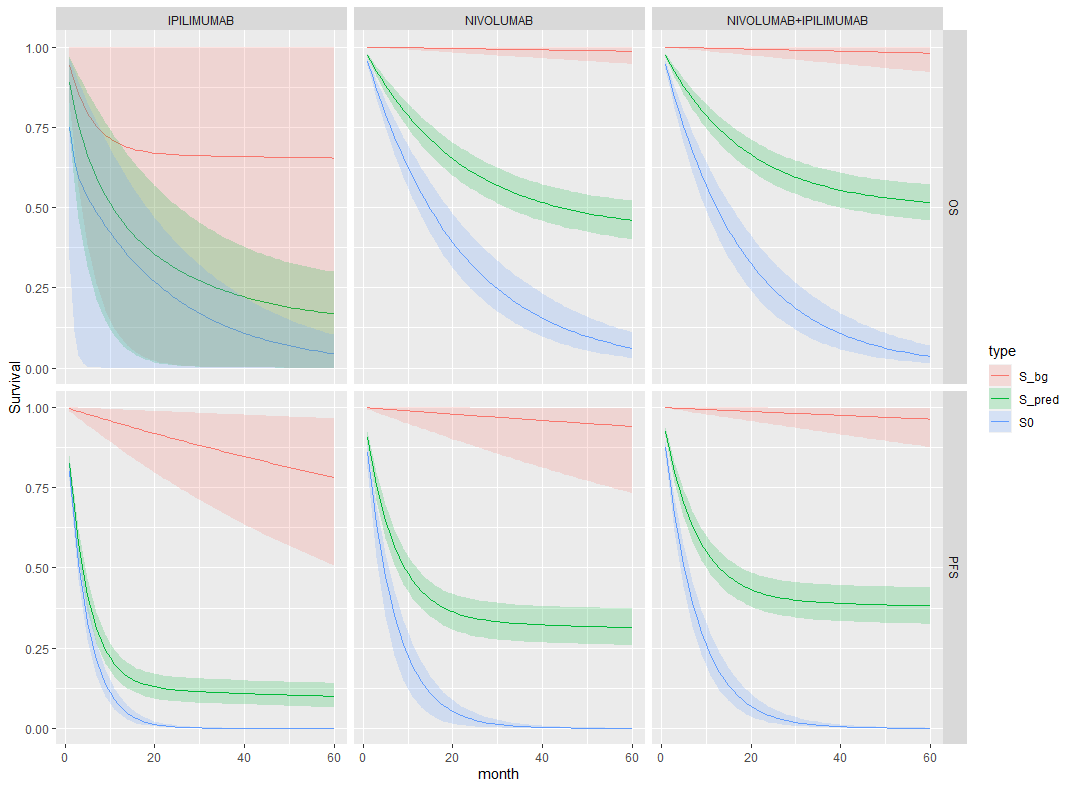
\includegraphics{../plots/exp_posterior_S_all.png}
\caption{Exponential hazard posterior survival}
\end{figure}

\begin{figure}
\centering
\includegraphics[width=0.5\textwidth,height=\textheight]{C:/Users/Nathan/Documents/mixture cure model project/from Antonio/BMS_ICON_cure_modeling/MCM_15012020/Figures/pfs_rates.png}
\caption{Frequentist approach}
\end{figure}

\begin{figure}
\centering
\includegraphics[width=0.5\textwidth,height=\textheight]{C:/Users/Nathan/Documents/mixture cure model project/from Antonio/BMS_ICON_cure_modeling/MCM_15012020/Figures/os_rates.png}
\caption{Frequentist approach}
\end{figure}

\end{document}
